\subsection{Behavior analysis}

As soon as the application was installed it would constantly give a popup telling the user to enable Chrome. 
It also will constantly open a window showing the user how to enable the app. 
If the user tries to force the app to close via these settings it will not work. 
The app will constantly open and force the user to enable the app until it is either uninstalled or enabled.
The popup contained instructions that showed how the user would be able to “enable chrome”. 
Touching anywhere on the screen would redirect the user to the Accessibility settings. 
In this menu it would be possible to enable chrome. What it would enable is however not shown on these settings. 
After the user had enabled this setting the application would disappear from the main menu and silently run in the background. 
The only way the user would be able to find this app would be in the application settings. 
In the application settings the app would still be shown as installed. 
Any attempts from the user to remove the app at this stage will be thwarted by the app.
This is shown on figure \ref{tim-appbehavior}

\begin{figure}[H]
    \centering
    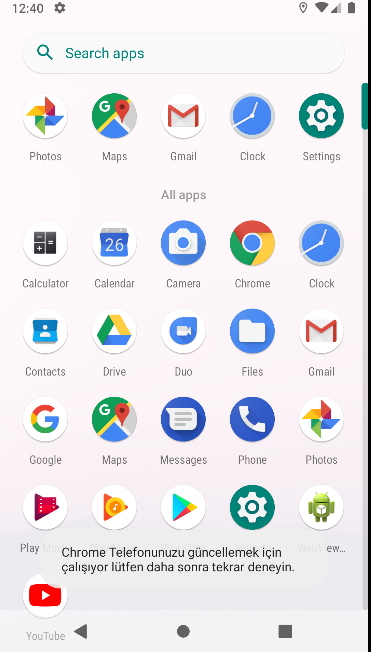
\includegraphics[width=5cm, height=16cm, keepaspectratio]{behaviorimg.png}
    \caption{app booting you from application settings}
    \label{tim-appbehavior}
\end{figure}

The message that the user will be met with when trying to edit the application settings of the malicious chrome translates to: 
Chrome is working to update your phone please try again later.
If the application has reached this stage it would be impossible to remove it from a normal phone.
